\section{Server}\label{section1}
Il Server è stato implementato in Java e utilizza il framework Javalin per mettersi in ascolto su una porta predefinita, accettando e gestendo le richieste HTTP provenienti dai Client. Tutte le interrogazioni in entrata sono sottoposte a un attento processo di analisi e filtraggio, al fine di garantire l'aderenza agli standard definiti dallo sviluppatore. Di fatto, qualsiasi richiesta che non sia conforme a tali standard viene prontamente ignorata e scartata per garantire la sicurezza e l'integrità del sistema.\\
Per essere considerata valida, una richiesta deve almeno includere il token di accesso o il token di aggiornamento nell header, a meno che non si tratti specificamente di una richiesta di accesso al sistema. In quest'ultimo caso, il processo di autenticazione viene innescato e, una volta completato con successo, il Server risponde inviando al Client i token di accesso e di aggiornamento, come precedentemente stabilito nella \Cref{subsub:twotoken} del presente elaborato.

\subsection{Database: Analisi e Struttura} \label{section2}
\begin{figure}
	\centering
	\makebox[\textwidth] [c]{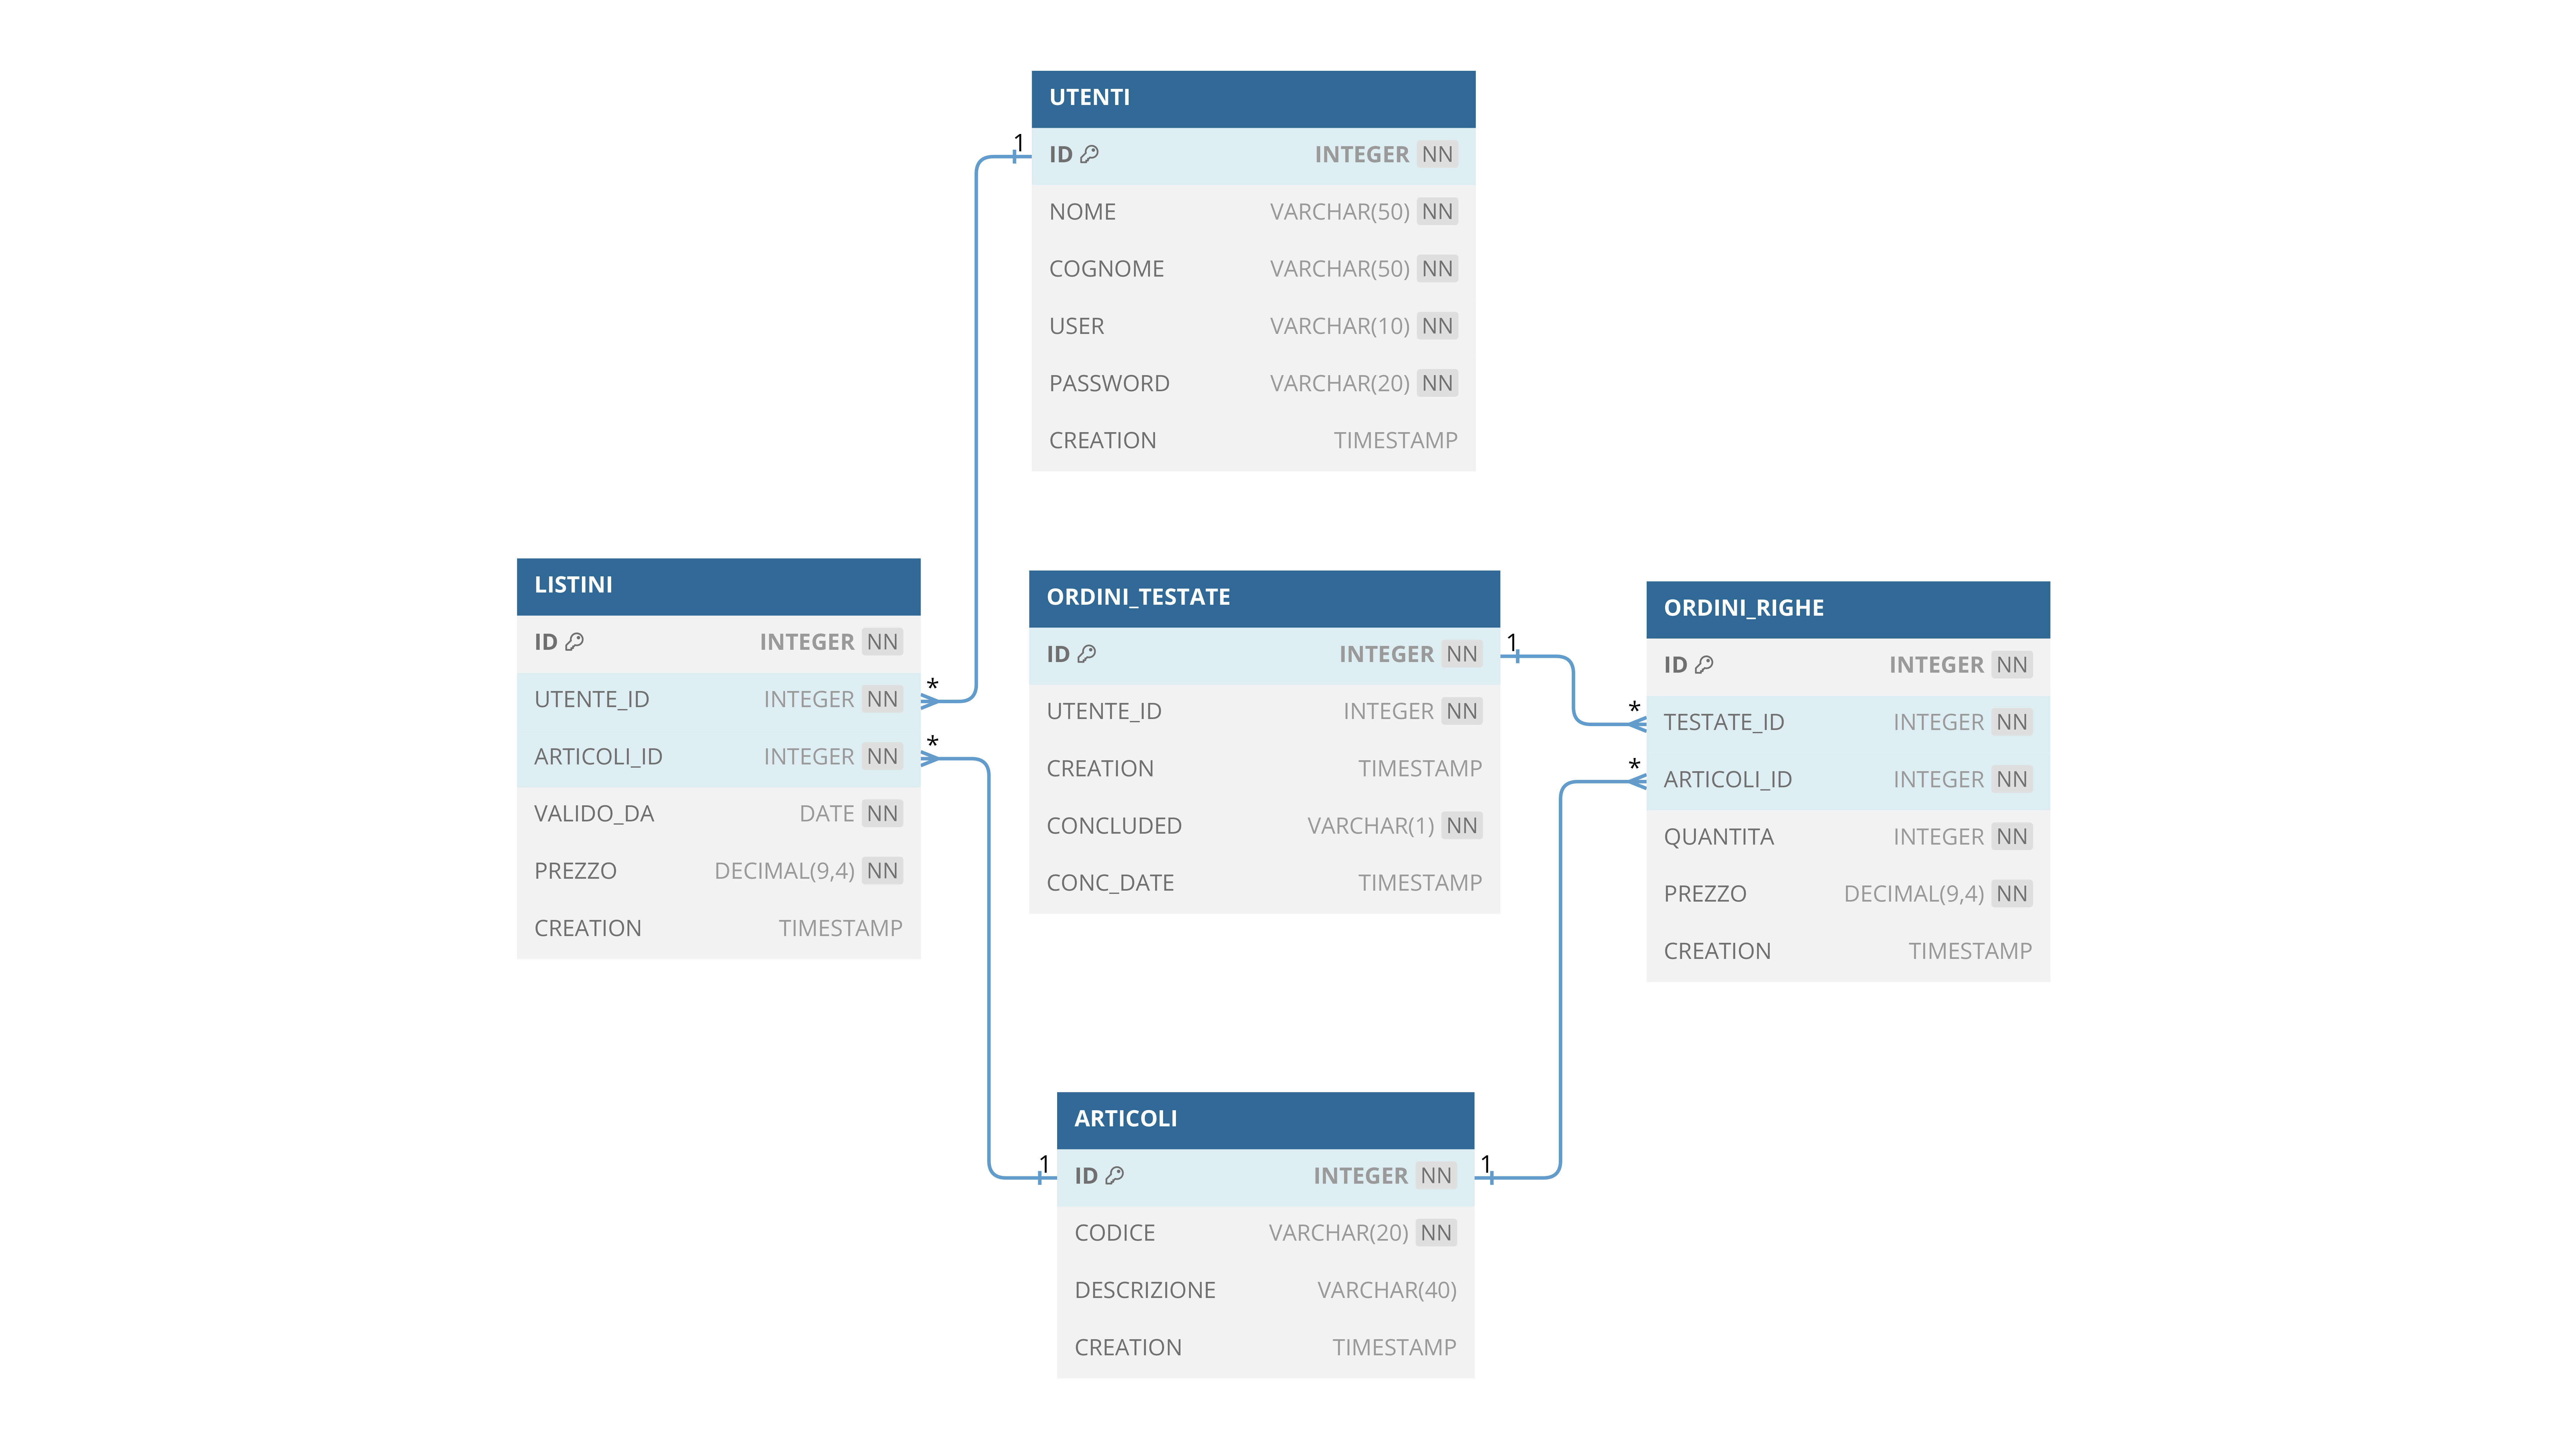
\includegraphics[width=1.6\linewidth, keepaspectratio]{Assets/dbdiagram.png}}
	\caption{Struttura del Database}
	\label{fig:dbdiagram}
\end{figure}

Nel diagramma illustrato in \Cref{fig:dbdiagram}, sono rappresentate le tabelle che costituiscono il Database, corredate delle rispettive chiavi esterne e primarie.\\
Particolarmente rilevante è la relazione tra le tabelle "UTENTI" e "ARTICOLI", che è di tipo molti-a-molti. Tale scelta deriva dalla necessità di assegnare un listino prezzi dedicato a ciascun cliente. Di conseguenza, un singolo utente può disporre di una pluralità di articoli con prezzi specifici, mentre un articolo può essere dedicato a numerosi utenti. Questo meccanismo permette di personalizzare l'esperienza dell'utente, fornendo tariffe e condizioni di vendita mirate.\\
La tabella "LISTINI" rappresenta l'insieme dei prezzi per prodotto dedicato a ciascun utente, di fatto tale approccio favorisce una gestione flessibile dei costi e promuove una maggiore adattabilità commerciale, consentendo di offrire politiche di prezzo diversificate.\\
Ulteriori relazioni rilevanti sono quelle tra le tabelle "ARTICOLI" e "ORDINI\_TESTATE". La relazione molti-a-molti tra queste due entità riflette la possibilità che un articolo possa essere acquistato da più utenti diversi (in sostanza che un articolo possa stare in più "carrelli"). D'altra parte, la tabella "ORDINI\_TESTATE" consente di raggruppare diversi articoli o prodotti all'interno di un singolo ordine. Ciò significa che un ordine può contenere una molteplicità di articoli, ognuno con la propria quantità e prezzo specifico (tutto questo salvato nella tabella ORDINI\_RIGHE), che viene ottenuto dalla tabella "LISTINI" come scritto in precedenza. In sostanza, quindi, ogni prodotto che un utente acquista ha un prezzo specifico dalla tabella LISTINI: quando il prodotto viene aggiunto al carrello, viene registrato nella tabella ORDINI\_RIGHE e il riferimento al carrello appena creato viene memorizzato nella tabella ORDINI\_TESTATE.

\subsubsection{Query}
Le query utilizzate per interrogare il Database possono variare a seconda della richiesta ricevuta. Durante la fase di login, il Client invia al Server sia lo username che la password inseriti dall'utente nell'applicazione, e di conseguenza, diventa indispensabile confrontare tali informazioni con quelle memorizzate nel Database. A tal fine, si impiega la seguente query:
\begin{lstlisting}[language=sql] [H]
	SELECT u.ID FROM UTENTI u 
	WHERE u.USER = 'user' AND u.PASSWORD = 'password'
\end{lstlisting}

\noindent
Una volta effettuato il login, l'utente ha la possibilità di ricercare prodotti attraverso l'apposita barra di ricerca. A tale scopo, il Client invia una richiesta specifica al Server contenente la parola chiave desiderata, con l'obiettivo di ottenere i prodotti corrispondenti e relativo prezzo. La risposta fornita dal Server, quindi, consiste in una lista di prodotti il cui nome contiene la parola chiave indicata, accompagnata dal relativo prezzo dedicato all'utente.\\
\\
Per effettuare questa operazione, viene utilizzata la seguente query:
\begin{lstlisting}[language=sql] [H]
	SELECT l.ARTICOLI_ID, a.DESCRIZIONE, l.PREZZO FROM UTENTI u
	INNER JOIN LISTINI l ON u.ID = l.UTENTE_ID
	INNER JOIN ARTICOLI a ON l.ARTICOLI_ID = a.ID 
	AND u.ID = id AND LOWER(a.DESCRIZIONE) LIKE '%keyword%'
\end{lstlisting}

\noindent
Per esempio, un possibile output ricercando la keyword "mele" è il seguente:
\begin{lstlisting}[language=json] [H]
	{
		"body":[
		{
			"id":1341,
			"name":"MELE RED DELIC 19K",
			"price":0.028,
			"quantity":0
		},
		{
			"id":1387,
			"name":"MELE RED DELIC 18K",
			"price":0.028,
			"quantity":0
		},
		{
			"id":1697,
			"name":"MELE RED DELIC 12K",
			"price":0.028,
			"quantity":0
		}
		]
	}
\end{lstlisting}

\noindent
Una volta individuato il prodotto desiderato, l'utente ha la possibilità di aggiungerlo al carrello mediante la creazione di una testata. Per compiere questa operazione, il Client invia una richiesta specifica al Server contenente il codice del prodotto e la quantità relativa (impostata di default a 1).
Successivamente, il Server verifica se il Client ha specificato la testata nell'header; nel caso in cui non sia stata specificata, il sistema procede a crearne una corrispondente per l'utente in questione. A tal scopo, si utilizza la seguente query (con parametri testataId, prodId, orderQuantity e userId):
\begin{lstlisting}[language=sql, firstnumber=1] [H]
	INSERT INTO ORDINI_TESTATE (UTENTE_ID) 
	SELECT ID FROM UTENTI WHERE ID = userId
\end{lstlisting}

\noindent
Se invece è specificata si controlla che non sia stata chiusa, che l'ordine non sia già stato inserito e in tal caso, se ne aumenta la quantità chiudendo la richiesta.
Le query sono rispettivamente:
\begin{lstlisting}[language=sql, firstnumber=1] [H]
	SELECT CONCLUDED FROM ORDINI_TESTATE WHERE ID = testataId
	
	SELECT * FROM ORDINI_RIGHE 
	WHERE TESTATE_ID = testataId AND ARTICOLI_ID = prodId;
	
	UPDATE ORDINI_RIGHE
	SET QUANTITA = orderQuantity
	WHERE TESTATE_ID = testataId AND ARTICOLI_ID = prodId;
\end{lstlisting}

\noindent
Nel caso in cui l'ordine venga inserito per la prima volta, esso verrà aggiunto nella tabella ORDINI\_RIGHE. Durante questo processo, verrà recuperato il prezzo corrispondente dalla tabella LISTINI utilizzando la seguente query:\footref{fn1}:
\begin{lstlisting}[language=sql, firstnumber=1] [H]
	INSERT INTO ORDINI_RIGHE 
	(TESTATE_ID, ARTICOLI_ID, QUANTITA, PREZZO)
	SELECT testataId, prodId, orderQuantity, l.PREZZO 
	FROM UTENTI u
	INNER JOIN LISTINI l ON u.ID = l.UTENTE_ID
	INNER JOIN ARTICOLI a ON l.ARTICOLI_ID = a.ID 
	AND u.ID = userId AND l.ARTICOLI_ID = prodId
\end{lstlisting}

\noindent
Infine il Client può richiedere di visualizzare il carrello con gli ordini aggiunti. In tal caso la query\footref{fn1} è la seguente:
\begin{lstlisting}[language=sql, firstnumber=1] [H]
	SELECT l.ARTICOLI_ID, a.DESCRIZIONE, l.PREZZO, o.QUANTITA
	FROM LISTINI l
	INNER JOIN ARTICOLI a ON l.ARTICOLI_ID = a.ID
	INNER JOIN ORDINI_RIGHE o ON a.ID = o.ARTICOLI_ID 
	WHERE o.TESTATE_ID = testataId AND l.UTENTE_ID = userId
\end{lstlisting}

\noindent
È stata altresì introdotta la possibilità di reperire informazioni sull'account utente, nonché di cancellare ordini dal carrello, concludere e chiudere testate. Queste funzionalità vengono gestite attraverso query semplici e di facile comprensione del tipo SELECT, UPDATE e DELETE, quindi evito di riportarle qui per risparmiare il lettore da una lettura superflua. L'unico accenno che mi sento di dare è sulla chiusura di una testata, la quale è possibile farla impostando ad 1 il campo CONCLUDED della tabella ORDINI\_TESTATE (immagine \ref{fig:dbdiagram}).

\subsection{Token: Come vengono generati e usati} \label{section_token}
Durante il ciclo di vita del Server, in determinati momenti, diventa essenziale acquisire l'id dell'utente che ha effettuato la richiesta, al fine di gestirla nel modo più adeguato. Di fatto, le query menzionate in precedenza impiegano ampiamente l'identificativo dell'utente (userId). Tuttavia, per motivi di sicurezza, questo "id" non può essere trasmesso tramite l'URI. Un primo approccio, quindi, che solitamente viene utilizzato quando si devono gestire degli utenti è tenere sul Server le informazioni necessarie, lette inizialmente dal Database, in una cache (solitamente rappresentata da una Map, nel mio caso una Map dove la chiave è il token e il valore è l'id utente) e interrogarla ogni qual volta sia necessario avere dati specifici. Tuttavia, questa metodologia può causare problemi di efficienza poiché la memorizzazione di tutte queste informazioni, per ciascun utente, può comportare un notevole aumento nell'utilizzo delle risorse e conseguentemente rallentare l'intero sistema in modo esponenziale.\\
I token JWT sono stati quindi pensati appositamente per rendere l'applicazione scalabile, facendo in modo che siano gli utenti a persistere sui loro dispositivi i dati necessari, affinché le loro richieste vengano gestite nella maniera più corretta. Grazie a questo approccio, non è più necessario utilizzare una cache sul Server, consentendo di liberare risorse e semplificare il mantenimento del Server.
Come descritto nel \Cref{subsub:secure}, la creazione dei token richiede l'utilizzo di una chiave simmetrica, usata per criptare i token JWT; la chiave e i token vengono quindi creati nel seguente modo:
\begin{lstlisting}[language=Java, firstnumber=1][H]
	
	/* Creazione della chiave */
	Key secretKey = Keys.secretKeyFor(SignatureAlgorithm.HS256);
	
	/* Metodo che genera un token firmato */
	public String generateToken(int userId) {
		return Jwts.builder()
		.setSubject(String.valueOf(userId))
		.setIssuer(ISSUER)
		.signWith(secretKey)
		.compact();
	}
\end{lstlisting}
\noindent
Durante la fase di accesso, l'id  dell'utente viene quindi estratto dal Database, inserito nel token JWT e, nei successivi invii di richieste, quest'identificatore verrà recuperato direttamente dal token, eliminando la necessità di consultare una cache.\\
Al fine di garantire l'autenticità e l'integrità dei token, evitando potenziali manomissioni da parte di Client malevoli, il Server adotta un metodo di verifica della firma del token mediante l'utilizzo della propria chiave simmetrica. Questo processo permette al Server di assicurarsi che il token sia valido e provenga da una fonte attendibile (cioè lui stesso!). Il metodo di verifica è il seguente:
\begin{lstlisting}[language=Java][H]
	/* Ritorna true se il token e' stato creato con secretKey, false altrimenti */
	public boolean isValid(String token) {
		try {
			Jwts.parserBuilder()
			.setSigningKey(secretKey)
			.requireIssuer(ISSUER)
			.setAllowedClockSkewSeconds(CLOCK_SKEW_SECONDS)
			.build()
			.parseClaimsJws(token);
			return true;
		}catch (JwtException e) {
			return false;
		}
	}
\end{lstlisting}

\noindent
Per verificare invece la sola scadenza del token, viene utilizzato il seguente metodo:
\begin{lstlisting}[language=Java][H]
	// Ritorna true se il token e' scaduto, false altrimenti
	public boolean isExpired(String token) {
		try {
			DecodedJWT jwt = JWT.decode(token);
			Date expirationDate = jwt.getExpiresAt();
			Date now = new Date();
			
			Calendar calendar = Calendar.getInstance();
			calendar.setTime(expirationDate);
			calendar.add(Calendar.SECOND, CLOCK_SKEW_SECONDS);
			expirationDate = calendar.getTime();
			
			return expirationDate.before(now);
		} catch (Exception e) {
			return true;
		}
	}
\end{lstlisting}

\noindent
E' facile intuire che questa chiave deve essere salvata da qualche parte al momento della sua creazione, in quanto la perdita di essa (per esempio al riavvio del Server) invaliderebbe tutti i token inviati ai Client, obbligandoli ad eseguire nuovamente il login.

\subsubsection{Creazione chiave e persistenza su disco} \label{subsub:key_creation_and_disk_persistency}
Per generare la chiave simmetrica viene impiegata la classe Keys della libreria JsonWebToken (vedi \Cref{sub:jwt}) nel seguente modo:
\begin{lstlisting}[language=Java, firstnumber=1][H]
	private Key generateKey() {
		return Keys.secretKeyFor(SignatureAlgorithm.HS256);
	}
\end{lstlisting}

\noindent
Tuttavia si è ritenuto poco sicuro salvarla semplicemente sul disco utlizzando la Serializzazione\cite{serializable} (essendo l'oggetto Key serializzabile) fornita da Java, quindi è stato deciso di criptarla mediante l'utilizzo di un altra chiave e scrivendone poi i byte cifrati sul disco rigido del Server. Per generare questa seconda chiave è necessario tuttavia avere una password, che di default ha valore pre-settato essendo in scopi didattici ma, in casi più normali, si sarebbe ad esempio chiesta all'avvio del Server o salvata su qualche disco sicuro.
Il procedimento è quindi:
\begin{enumerate}
	\item Convertire la password da tipo String a SecretKey
	\begin{lstlisting}[language=Java, firstnumber=1][H]
private SecretKey getPasswordKey(String password) {
	try {
		byte[] key = 
		password.getBytes(StandardCharsets.UTF_8);
				
		MessageDigest md = MessageDigest.getInstance("SHA-256");
				
		key = md.digest(key);
		return new SecretKeySpec(key, "AES");
				
	} catch (NoSuchAlgorithmException e) {
		e.printStackTrace();
	}
			
	throw new Exception("password exception");
}
	\end{lstlisting}
	
	\item Usare la SecretKey definita nel punto 1. per reperire la chiave dal disco. Il metodo definito sotto ritorna "null" in caso non esista alcuna chiave sul disco, o la Key in caso questa si trovi nella cartella definita dalla variabile globale "KEY\_PATH"
	\begin{lstlisting}[language=Java][H]
private Key readKeyFromFile(SecretKey passwordKey) {
	Path path = Path.of(KEY_PATH);
	if(Files.exists(path)) {
		byte[] encryptedMsg = Files.readAllBytes(path);
		
		byte[] decrypted = 
		decrypt(encryptedMsg, passwordKey);
		
		// Crea una nuova Key usando l'algoritmo HMAC-SHA
		return Keys.hmacShaKeyFor(decrypted);
	}
	
	return null;
}

byte[] decrypt(byte[] message, SecretKey passwordKey) {
	try {
		Cipher cipher = 
		Cipher.getInstance("AES/ECB/PKCS5PADDING");
		
		cipher.init(Cipher.DECRYPT_MODE, passwordKey);
		return cipher.doFinal(message);
	} catch (Exception e) {
		e.printStackTrace();
	}
	
	throw new Exception("Error while decrypting");
}
	\end{lstlisting}
	\item Se questa non è presente ne genero una nuova, ne vengono cifrati i byte usando la password e infine salvato il risultato sul disco
	\begin{lstlisting}[language=Java][H]
		Key secretKey = generateKey();
		
		private void writeKeyToFile(SecretKey passwordKey) 
		throws Exception {
			byte[] message = secretKey.getEncoded();
			
			byte[] encryptedMsg = encrypt(message, passwordKey);
			Files.write(Path.of(KEY_PATH), encryptedMsg);
		}
		
		private byte[] encrypt(byte[] message, SecretKey passwordKey) 
		throws Exception {
			try {
				Cipher cipher = 
				Cipher.getInstance("AES/ECB/PKCS5Padding");
				
				cipher.init(Cipher.ENCRYPT_MODE, passwordKey);
				return cipher.doFinal(message);
			} catch (Exception e) {
				e.printStackTrace();
			}
			
			throw new Exception("Error while crypting");
		}
		
	\end{lstlisting}
	
	\item Al riavvio del Server, ripartire dal punto numero 1
\end{enumerate}


\newpage
\noindent
Tutto questo si può riassumere quindi in:
\begin{lstlisting}[language=Java][H]
	SecretKey passwordKey = getPasswordKey(password);
	Key secretKey = readKeyFromFile(passwordKey);
	
	if (secretKey == null) {
		secretKey = generateKey();
		
		writeKeyToFile(passwordKey);
	}
\end{lstlisting}

\noindent
Più nello specifico, per generare la chiave dalla password viene ottenuta un'istanza dell'algoritmo hash SHA-256 attraverso la classe MessageDigest. SHA-256 è una funzione di hashing crittografica che restituisce un valore hash di 256 bit.\\
Per la criptazione e decriptazione viene usata la classe Cipher della libreria standard di Java, la quale viene impostata in modo che vengano usati gli algoritmi di AES, ECB e PKCS5Padding come descritto nella \Cref{subsub:secure}.

\subsection{Comunicare con il Server e Gestione delle\\ richieste tramite Javalin}\label{subsub:javalin}
Come descritto nella \Cref{section1}, il Server è stato implementato mediante l'utilizzo del framework Javalin il quale, al momento dell'avvio, crea un'istanza della classe Javalin utilizzando una porta predefinita, secondo queste modalità:
\begin{lstlisting}[language=Java, firstnumber=1][H]
	Javalin app = Javalin.create().start(7777);
\end{lstlisting}


\noindent
In seguito, si procede alla definizione delle rotte dell'applicazione: queste rappresentano gli endpoint del Server che successivamente si definiranno tramite delle URI. Le rotte vengono specificate mediante l'uso dei metodi HTTP come GET, POST, DELETE, eccetera, e richiedono l'inserimento di una callback (con un parametro context di tipo Context per eseguire diverse azioni, tra cui parsing del path o accesso all header) che verrà invocata quando un Client eseguirà una richiesta HTTP verso quella specifica route. Nel contesto di Javalin, per creare una route, ad esempio una route di tipo GET, si utilizza la seguente sintassi:

\begin{lstlisting}[language=Java]
	context.get("uri", context -> {
		// gestione della richiesta..
	});
\end{lstlisting}

\noindent
Per definire una route che richiede un parametro, si utilizza invece il seguente approccio:
\begin{lstlisting}[language=Java]
	context.get("/{param}", context -> {
		String value = context.pathParam("param");
		// gestisci la richiesta usando value..
	});
\end{lstlisting}

\noindent
In sostanza le routes costituiscono il meccanismo chiave per consentire l'interazione tra il Server e i Client.
Nel mio caso quindi le rotte sono le seguenti:
\begin{lstlisting}[language=Java, firstnumber=5][H]
	app.get("/users/login/{username}={password}", context -> {})
	app.get("/users/profile", context -> {})
	app.get("/users/logout", context -> {})
	app.get("/search/desc={desc}", context -> {})
	app.get("/search/code={code}", context -> {})
	app.get("/testata/{tid}", context -> {})
	app.get("/testata/{tid}/cart", context -> {})
	app.post("/orders/add={pid}&quantity={qt}", context -> {})
	app.post("/orders/add={pid}", context -> {})
	app.post("/orders/quantity/{pid}={q}", context -> {})
	app.post("/orders/complete", context -> {})
	app.delete("/orders/remove={pid}", context -> {})
\end{lstlisting}
\noindent
Il meccanismo di gestione delle richieste si basa quindi sull'estrapolare i valori passati come parametri dall'URI, costruire una query in base alla natura della richiesta (come descritto nella \Cref{section2}), ed eseguire tale query per ottenere i dati desiderati. Il Server risponderà al Client restituendo un oggetto JSON contenente il risultato ottenuto o un messaggio di errore in caso di problematiche.
È fondamentale notare che la maggior parte delle richieste deve includere il token di accesso (per ottenere l'ID utente, come illustrato nella \Cref{section_token}), e in alcuni casi, potrebbe essere richiesto anche l'ID della testata (ad esempio, quando si intende aggiungere un prodotto al carrello, come dettagliato nella \Cref{section2}).

\subsubsection{Messaggi di errore}
Durante il ciclo di vita dell'applicazione, può capitare che il Server debba restituire messaggi di errore: questi messaggi sono sempre in JSON e seguono il seguente formato:
\begin{lstlisting}[language=JSON, firstnumber=1][H]
	{
		"code": codice numerico rappresentativo dell'errore,
		"message": "Messaggio testuale esplicativo del codice"
	}
\end{lstlisting}